
\subsection{Estimation des coûts}

Nous indiquons ici le temps dédié à chacune des étapes du projet des deux sous-groupes suivi du temps consacré à la mise en commun de ces deux sous-parties.

\subsubsection{Automates}

\begin{flushleft}
\begin{tabular}{|l|c|r|}
  \hline
   Étape & Volume horaire \\
  \hline
  Travail initial sur les fichiers .an & 4h \\
     \hline
  Expressions régulières & 6h \\
  \hline
  Représentations visuelles des automates avec p5.js & 12h\\
  \hline
    Passage aux courbes de Bézier & 4h \\
  \hline
    Déplacement des arcs avec onmouse & 8h\\
  \hline
   Prise en main et calcul des overBox  & 6h \\
  \hline
   Affichage des transitions avec mousePressed() & 8h \\
    \hline
 \end{tabular}
 \end{flushleft}

Au total, nous avons consacré environ \textbf{48} heures pour cette sous-partie. 

\subsubsection{Graphes}

\begin{flushleft}
\begin{tabular}{|l|c|r|}
  \hline
   Étape & Volume horaire \\
  \hline
  Réalisation des fenêtres & 15h \\
     \hline
  Parser & 5h \\
  \hline
  Dessin du graphe & 2h \\
  \hline
  Légende interactive & 7h \\
  \hline
  Sélection des jeux de données dans le fichier tsv & 1h \\
  \hline
  RangeSlider & 6h \\
  \hline
  Affichage des seuils & 3h \\
  \hline
  Curseur temporel & 3h \\
  \hline
  Graphismes, ergonomie & 3h\\
  \hline
  
 \end{tabular}
 \end{flushleft}

Au total, nous avons consacré environ \textbf{45} heures pour cette sous-partie. 
  
\subsubsection{Mise en commun}

\begin{flushleft}
\begin{tabular}{|l|c|r|}
  \hline
   Étape & Volume horaire \\
  \hline
  Montée en connaissance sur javascript & 10h \\
  \hline
  Transfert des données & 5h \\
    \hline
 Rédaction du rapport & 6h \\
 \hline
    
 \end{tabular}
 \end{flushleft}

Au total, nous avons consacré environ \textbf{21} heures pour cette sous-partie.
\bigbreak
Ainsi, ce projet de groupe a été réalisé en \textbf{114} heures de travail. 
  
  
\bigbreak
\bigbreak
\subsection{Difficultés rencontrées}
\bigbreak

\subsubsection{Récupération des données depuis les fichiers .an}
Concernant la partie automates, notre première difficulté fut de récupérer les données des automates à partir des fichiers .an fournis:

\begin{figure}[!h]
  \centering
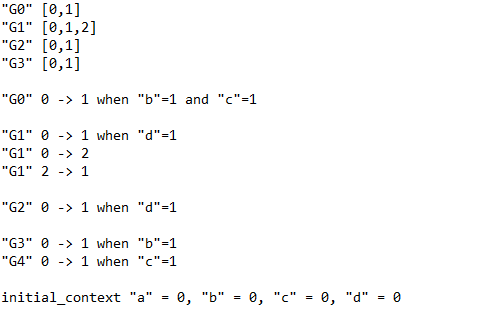
\includegraphics[scale = .7]{images/fichier_an.png} 
\caption{Exemple de fichier .an}
\end{figure}
Au départ, nous avions opté pour la méthode naïve de lire chacune des lignes et d’utiliser la méthode split (selon ”when”, ”and” et ”-”) mais cette méthode a rapidement montré ses limites. En effet, elle cesse de fonctionner dès lors qu’il y a plus de 10 automates puisque avoir ”G10” au lieu de ”G9” décalerait d’une case notre récupération naïve.
Nous avons alors décidé d’abandonner cette méthode et avons préféré utiliser des expressions régulières permettant une lecture bien plus robuste que la précédente.

\bigbreak
\subsubsection{Affichage des transitions}

Le dernier obstacle majeur de la partie automates a été celui de l’affichage dynamique des transitions. En effet, nous voulions initialement que l’affichage d’une transition ne se fasse que lorsque l’utilisateur survole avec sa souris l'etat initial concerné. Nous avons alors dû consacrer beaucoup de temps pour trouver une solution parmi la documentation souvent très absconse de p5.js et il a fallu réécrire cette fonctionnalité à chaque fois que la représentation visuelle des automates et de leurs arcs a été changée. Nous avions finalement retenu le principe de l’overBox qui construisait un périmètre autour de l’arc et affichait la transition dès lors que l’utilisateur passait la souris dans ce périmètre. Cependant, lors de notre réunion finale, il a été décidé que cette fonctionnalité n’était plus voulue et qu’un affichage permanent de toutes les transitions était préférable, c’est pourquoi nous l’avons enlevée.

\bigbreak
\subsubsection{Le manque de documentation de grafica}
\bigbreak
Nous avons retenu cette librairie car elle fonctionne grâce à p5 qui est déjà inclus dans la page et propose les fonctionnalités dont nous avions besoin pour ViMaSTBio. En revanche, le code est très peu commenté et aucune documentation n’est fournie, que ce soit sur la page github du projet ou sur le site de la librairie. Heureusement, ce même site proposait quelques applications possibles grâce auxquelles nous avons pu comprendre son fonctionnement. En revanche, nous avons dû fouiller dans le code pour chercher les fonctions supplémentaires dont nous avions besoin, ce qui a bien ralenti le développement de l’outil.
\bigbreak

\subsubsection{La montée en compétences sur JavaScript}
\bigbreak

Personne n’avait pratiqué le JavaScript avant ce projet parmi nous. Or ce langage possède quelques particularités incontournables dans son fonctionnement telles que les prototypes - des hybrides entre les objets et les classes qui sont d’ailleurs absents, un typage faible et dynamique qui ne permet pas une visualisation claire du contenu des variables ou encore le mécanisme des callbacks lorsqu’on fait de l’AJAX (Asynchronous Javascript And Xml) comme dans le chargement des fichiers.

L’ensemble de ces facteurs a encore une fois contribué à ralentir notre avancée lorsque nous étions confrontés à des comportements imprévus du fait de notre manque de pratique du JavaScript.
